\documentclass[12pt,a4paper,twoside,spanish]{article}      % Libro a 11 pt
\usepackage[utf8]{inputenc}
\usepackage[height=17.5cm,width=13.5cm]{geometry}
\usepackage[spanish]{babel}         % diccionario
\usepackage{epsfig}         % Graficos Postscript
\usepackage{tabularx}
\usepackage{sectsty}
\usepackage{graphicx}
\usepackage{float}
\graphicspath{ {./images/} }


%%%%%%%%%%%%%%%%%%%%%%%%%%%%%%%%%%%%%%%%%%%%%%%
%%%%%%%%%%%%%
%%%%%%%%%%%%% Margenes
%%%%%%%%%%%%%
%%%%%%%%%%%%%%%%%%%%%%%%%%%%%%%%%%%%%%%%%%%%%%%
%%%%% Definimos el maximo tamaño posible.
\marginparwidth 0pt     \marginparsep 0pt
\topmargin   0pt        \textwidth   6.5in
\textheight 23cm

% Margen izq del txt en impares.
\setlength{\oddsidemargin}{.0001\textwidth}

% Margen izq del txt en pares.
\setlength{\evensidemargin}{-.04\textwidth}

% Anchura del texto
\setlength{\textwidth}{.99\textwidth}


%%%%%%%%%%%%%%%%%%%%%%%%%%%%%%%%%%%%%%%%%%%%%%%
%%%%%%%%%%%%%
%%%%%%%%%%%%% Profundidad de enumeracion y tabla de contenidos
%%%%%%%%%%%%%
%%%%%%%%%%%%%%%%%%%%%%%%%%%%%%%%%%%%%%%%%%%%%%%

\setcounter{secnumdepth}{3}
\setcounter{tocdepth}{3}


%%%%%%%%%%%%%%%%%%%%%%%%%%%%%%%%%%%%%%%%%%%%%%%
%%%%%%%%%%%%%
%%%%%%%%%%%%% Nuevos Comandos
%%%%%%%%%%%%%
%%%%%%%%%%%%%%%%%%%%%%%%%%%%%%%%%%%%%%%%%%%%%%%

            %%%%%%%%%%%%%%%%%%%%%%%
            %%%%%%%%%%%%%%%%%%%%%%%
            % Comandos para simplificar
            % la escritura
            %%%%%%%%%%%%%%%%%%%%%%%
            %%%%%%%%%%%%%%%%%%%%%%%

\def\mc{\multicolumn}
            %%%%%%%%%%%%%%%%%%%%%%%
            % Comandos para poder utilizar raggedright en tablas
            %%%%%%%%%%%%%%%%%%%%%%%
\newcommand{\PreserveBackslash}[1]{\let\temp=\\#1\let\\=\temp}
\let\PBS=\PreserveBackslash




%%%%%%%%%%%%%%%%%%%%%%%%%%%%%%%%%%%%%%%%%%%%%%%
%%%%%%%%%%%%%
%%%%%%%%%%%%% Cuerpo del documento
%%%%%%%%%%%%%
%%%%%%%%%%%%%%%%%%%%%%%%%%%%%%%%%%%%%%%%%%%%%%%


\begin{document}

\def\chaptername{Capítulo}
\def\tablename{Tabla}
\def\listtablename{Índice de Tablas}
\chapterfont{\LARGE\raggedleft}

%%%%%%%%%%%%%%%%%%%%%%%%%%%%%%%%%%%%%%%%%%%%%%%%%%%%%%%%%%%%%%%
%%%%%%%%%%%%%%%%%%%%%%%%%%%%%%%%%%%%%%%%%%%%%%%%%%%%%%%%%%%%%%%
% DISEÑO DE LA PAGINA DEL TITULO
%%%%%%%%%%%%%%%%%%%%%%%%%%%%%%%%%%%%%%%%%%%%%%%%%%%%%%%%%%%%%%%
%%%%%%%%%%%%%%%%%%%%%%%%%%%%%%%%%%%%%%%%%%%%%%%%%%%%%%%%%%%%%%%
\pagestyle{empty}

\begin{titlepage}
\setlength{\parindent}{0cm} \setlength{\parskip}{0cm}

%\raggedleft {\textsf{\textbf{Login del grupo: xxxx}}}

\newcommand{\HRule}{\rule{\linewidth}{1mm}}

\vspace*{2cm}
\HRule \\[0.5cm]
\begin{center}
% Letra lineal y negrita
\textsf{\textbf{\large UN SISTEMA BASADO EN CONOCIMIENTO PARA \ldots(LA PLANIFICACIÓN Y ENTRENAMIENTO DEL KARATE)\\[0.75cm] MODELADO CONCEPTUAL EN COMMONKADS \\[0.5cm]}}
\HRule \vspace*{3cm}

\textsf{\textbf{\normalsize Daniel Gago Martínez, Manuel Santamariña Ruiz de León, Daniel Deza Prieto, Hugo García\\[5cm]
Horario de prácticas: 3.1\\
Login de entrega: \\[2.5cm]
Desarrollo de Sistemas Inteligentes\\
Universidade da Coruña \\ Curso
202X}}
\end{center}
\end{titlepage}

\cleardoublepage

%%%%%%%%%%%%%%%%%%%%%%%%%%%%%%%%%%%%%%%%%%%%%%%
%%
%% TABLA DE CONTENIDOS
%%
%%%%%%%%%%%%%%%%%%%%%%%%%%%%%%%%%%%%%%%%%%%%%%%

\pagenumbering{Roman}
\tableofcontents
\cleardoublepage


%%%%%%%%%%%%%%%%%%%%%%%%%%%%%%%%%%%%%%%%%%%%%%%%%%%%%%%%%%%%%%%
%%%%%%%%%%%%%%%%%%%%%%%%%%%%%%%%%%%%%%%%%%%%%%%%%%%%%%%%%%%%%%%
%CONTENIDO DEL DOCUMENTO
%%%%%%%%%%%%%%%%%%%%%%%%%%%%%%%%%%%%%%%%%%%%%%%%%%%%%%%%%%%%%%%
%%%%%%%%%%%%%%%%%%%%%%%%%%%%%%%%%%%%%%%%%%%%%%%%%%%%%%%%%%%%%%%

%numeros arábigos
\pagenumbering{arabic} \pagestyle{myheadings} \markboth{Grupo de
prácticas: xxx}{Modelado Conceptual en CommonKADS.}

%indentaciones y espaciado entre párrafos
\setlength{\parindent}{1,5cm} \setlength{\parskip}{0,7cm}


%%%%%%%%%%%%%%%%%%%%%%%%%%%%%%%%%%%%%%%%%%%%%%%%%%%%%%%%%%%%%%%
%% BORRAR
%%%%%%%%%%%%%%%%%%%%%%%%%%%%%%%%%%%%%%%%%%%%%%%%%%%%%%%%%%%%%%%


%%%%%%%%%%%%%%%%%%%%%%%%%%%%%%%%%%%%%%%%%%%%%%%%%%%%%%%%%%%%%%%%%%%%%%%%%%%%%%%
\section{Modelo de Conocimiento.}
%%%%%%%%%%%%%%%%%%%%%%%%%%%%%%%%%%%%%%%%%%%%%%%%%%%%%%%%%%%%%%%%%%%%%%%%%%%%%%%

%%Se deberá entregar la documentación correspondiente a las tres fases
%%de diseño del modelo (explicadas en el capítulo 7 del libro de Shreiber).

%%%%%%%%%%%%%%%%%%%%%%%%%%%%%%%%%%%%%%%%%%%%%%%%%%%%%%%%%%%%%%%%%%%%%%%%%%%%%%%
\subsection{Fase de Identificación}
%%%%%%%%%%%%%%%%%%%%%%%%%%%%%%%%%%%%%%%%%%%%%%%%%%%%%%%%%%%%%%%%%%%%%%%%%%%%%%%
Para este SBC nos centraremos en la tarea 3, Planificación.

        \begin{table}[H]
            \scriptsize
            \begin{tabularx}{\textwidth}{|l|X|} \hline       
                \textbf{Modelo de Tareas} & \textbf{Formulario TM-1: Análisis de Tareas} \\ \hline\hline
                
                \textsc{Tarea} & T3 – Planificación del entrenamiento (Ref. OM-3) \\ \hline
                
                \textsc{Organización}  & Proceso central del dojo bajo responsabilidad técnica del Sensei. \\ \hline
                
                \textsc{Objetivo y valor} & Diseñar sesiones estructuradas que permitan alcanzar los objetivos definidos. Aporta organización y eficiencia. \\ \hline
                
                \textsc{Dependencia y Flujos} 
                & \textit{1. Tareas precedentes:} T2 – Definición de objetivos.\\
                & \textit{2. Tareas que le siguen:} T4 – Seguimiento del progreso. \\ \hline
                
                \textsc{Objetos manipulados} 
                & 1. Entrada: objetivos definidos.\\
                & 2. Salida: plan de entrenamiento estructurado.\\
                & 3. Internos: heurísticas y principios de planificación (OM-4). \\ \hline
                
                \textsc{Tiempo y control} 
                & 1. Frecuencia: periódica (mensual o por ciclo).\\
                & 2. Control: determina ejecución de sesiones.\\
                & 3. Restricciones: equilibrio entre carga y recuperación. \\ \hline
                
                \textsc{Agentes} & Sensei. \\ \hline
                
                \textsc{Conocimiento y Capacidad} & Uso intensivo de heurísticas y principios deportivos (OM-4). Tarea altamente intensiva en conocimiento. \\ \hline
                
                \textsc{Recursos} & Tiempo del Sensei, material del dojo. \\ \hline
                
                \textsc{Calidad y eficiencia} & Coherencia del plan y progresión técnica observada. \\ \hline
            \end{tabularx}
            \label{tab.TM1-T3}
          \end{table}
          \begin{table}[H]
            \scriptsize
            \begin{tabularx}{\textwidth}{|p{5cm}|>{\PBS\raggedright}p{0.8cm}|X|} \hline
                \textbf{Modelo de Tareas} & \multicolumn{2}{l|}{\textbf{Formulario TM-2: Elemento de Co\-no\-ci\-mien\-to}} \\ \hline\hline

                \textsc{Nombre} &  \multicolumn{2}{l|}{Principios de planificación}\\ \hline

                \textsc{Poseído por} &  \multicolumn{2}{X|}{Sensei}\\ \hline

                \textsc{Usado en} &  \multicolumn{2}{l|}{Tarea 3 – Planificación del entrenamiento}\\ \hline

                \textsc{Dominio} &  \multicolumn{2}{p{7.5cm}|}{\textbf{Rama:} Gestión y planificación del entrenamiento deportivo}\\ \hline

                \textbf{Naturaleza del conocimiento} & \emph{(Sí/No)} &
                \textbf{¿Supone un cuello de botella?¿Debe ser mejorado?}\\ \hline 

                Formal, riguroso & No & Si, muchas planificaciones se hacen de forma intuitiva sin seguir un procedimiento estructurado \\ \hline 

                Empírico, cuantitativo& No & No\\ \hline

                Heurístico, sentido común& Si & No\\ \hline

                Altamente especializado, específico del dominio& Si & No\\ \hline 

                Basado en la experiencia& Si & No\\ \hline 

                Basado en la acción$^1$& Si & No\\ \hline

                Incompleto& Si & No\\\hline 

                Incierto, puede ser incorrecto & Si & Si, pueden cometerse errores al olvidar factores de planificación \\ \hline 

                Cambia con rapidez& No  & No\\ \hline 

                Difícil de verificar& Si & Si, no siempre es sencillo evaluar si una planificación es óptima \\ \hline 

                Tácito, difícil de transferir& Si & Si, depende mucho de la experiencia del instructor \\ \hline 

                \textbf{Forma del conocimiento} & &\\ \hline

                Mental& Si & Si, gran parte del conocimiento se mantiene en la experiencia del Sensei \\ \hline

                Papel& Si & Si, realizarlo manualmente puede ser laborioso \\ \hline 

                Electrónica& No  & Si, podría formalizarse mediante el sistema experto \\ \hline

                Habilidades&Si  & No\\ \hline 

                Otros& No & No\\ \hline 

                \textbf{Disponibilidad del Conocimiento} &  &\\ \hline 

                Limitaciones en tiempo& Si  & Si, al planificar rápidamente pueden omitirse detalles \\ \hline

                Limitaciones en espacio& No & No \\ \hline 

                Limitaciones de acceso& Si & No \\ \hline 

                Limitaciones de calidad& Si & No \\ \hline 

                Limitaciones de forma& Si & Si, el conocimiento no está formalizado en reglas claras \\ \hline

            \end{tabularx}
            \label{tab.TM2}
        \end{table}
        \begin{table}[H]
            \scriptsize
            \begin{tabularx}{\textwidth}{|p{5cm}|>{\PBS\raggedright}p{0.8cm}|X|} \hline
                \textbf{Modelo de Tareas} & \multicolumn{2}{l|}{\textbf{Formulario TM-2: Elemento de Co\-no\-ci\-mien\-to}} \\ \hline\hline

                \textsc{Nombre} &  \multicolumn{2}{l|}{Reglas de carga-descanso}\\ \hline

                \textsc{Poseído por} &  \multicolumn{2}{X|}{Sensei}\\ \hline

                \textsc{Usado en} &  \multicolumn{2}{l|}{Tarea 3 – Planificación del entrenamiento}\\ \hline

                \textsc{Dominio} &  \multicolumn{2}{p{7.5cm}|}{\textbf{Rama:} Ciencias del deporte / preparación física}\\ \hline

                \textbf{Naturaleza del conocimiento} & \emph{(Sí/No)} &
                \textbf{¿Supone un cuello de botella?¿Debe ser mejorado?}\\ \hline 

                Formal, riguroso & No & Si, las reglas se aplican de forma aproximada sin un procedimiento formal claro \\ \hline 

                Empírico, cuantitativo& Si & No\\ \hline

                Heurístico, sentido común& Si & No\\ \hline

                Altamente especializado, específico del dominio& Si & No\\ \hline 

                Basado en la experiencia& Si & No\\ \hline 

                Basado en la acción$^1$& Si & No\\ \hline

                Incompleto& Si & Si, pueden faltar datos sobre recuperación o fatiga del alumno\\\hline 

                Incierto, puede ser incorrecto & Si & Si, una mala estimación puede provocar sobreentrenamiento\\ \hline 

                Cambia con rapidez& No & No\\ \hline 

                Difícil de verificar& Si & No\\ \hline 

                Tácito, difícil de transferir& Si & Si, depende mucho de la experiencia del Sensei \\ \hline 

                \textbf{Forma del conocimiento} & &\\ \hline

                Mental& Si & Si, gran parte del conocimiento se aplica de memoria\\ \hline

                Papel& No & No\\ \hline 

                Electrónica& No  & Si, podría registrarse para facilitar la planificación\\ \hline

                Habilidades&Si  & No\\ \hline 

                Otros& No & No\\ \hline 

                \textbf{Disponibilidad del Conocimiento} &  &\\ \hline 

                Limitaciones en tiempo& Si  & Si, durante la planificación rápida puede omitirse algún ajuste\\ \hline

                Limitaciones en espacio& No & No \\ \hline 

                Limitaciones de acceso& Si & Si, depende del conocimiento del instructor \\ \hline 

                Limitaciones de calidad& Si & No \\ \hline 

                Limitaciones de forma& Si & Si, no está formalizado en reglas claras \\ \hline
            \end{tabularx}
            \label{tab.TM2}
        \end{table}


        \begin{table}[H]
            \scriptsize
            \begin{tabularx}{\textwidth}{|p{5cm}|>{\PBS\raggedright}p{0.8cm}|X|} \hline
                \textbf{Modelo de Tareas} & \multicolumn{2}{l|}{\textbf{Formulario TM-2: Elemento de Co\-no\-ci\-mien\-to}} \\ \hline\hline

                \textsc{Nombre} &  \multicolumn{2}{l|}{Criterios técnicos por cinturón}\\ \hline

                \textsc{Poseído por} &  \multicolumn{2}{X|}{Sensei}\\ \hline

                \textsc{Usado en} &  \multicolumn{2}{l|}{Tarea 1 – Evaluación inicial, Tarea 5 – Evaluación de resultados}\\ \hline

                \textsc{Dominio} &  \multicolumn{2}{p{7.5cm}|}{\textbf{Rama:} Técnica y pedagogía del karate}\\ \hline

                \textbf{Naturaleza del conocimiento} & \emph{(Sí/No)} &
                \textbf{¿Supone un cuello de botella?¿Debe ser mejorado?}\\ \hline 

                Formal, riguroso & Si & No \\ \hline 

                Empírico, cuantitativo& No & No\\ \hline

                Heurístico, sentido común& Si & No\\ \hline

                Altamente especializado, específico del dominio& Si & No\\ \hline 

                Basado en la experiencia& Si & No\\ \hline 

                Basado en la acción$^1$& Si & No\\ \hline

                Incompleto& No & No\\\hline 

                Incierto, puede ser incorrecto & Si & Si, la evaluación técnica puede ser subjetiva\\ \hline 

                Cambia con rapidez& No & No\\ \hline 

                Difícil de verificar& Si & Si, la valoración puede variar entre instructores\\ \hline 

                Tácito, difícil de transferir& Si & No \\ \hline 

                \textbf{Forma del conocimiento} & &\\ \hline

                Mental& Si & Si, el Sensei suele aplicar estos criterios de memoria\\ \hline

                Papel& Si & No\\ \hline 

                Electrónica& No  & No\\ \hline

                Habilidades&Si  & No\\ \hline 

                Otros& No & No\\ \hline 

                \textbf{Disponibilidad del Conocimiento} &  &\\ \hline 

                Limitaciones en tiempo& No  & No\\ \hline

                Limitaciones en espacio& No & No \\ \hline 

                Limitaciones de acceso& Si & No \\ \hline 

                Limitaciones de calidad& Si & Si, depende de la experiencia del instructor \\ \hline 

                Limitaciones de forma& Si & No \\ \hline

            \end{tabularx}
            \label{tab.TM2}
        \end{table}


        \begin{table}[H]
            \scriptsize
            \begin{tabularx}{\textwidth}{|p{5cm}|>{\PBS\raggedright}p{0.8cm}|X|} \hline
                \textbf{Modelo de Tareas} & \multicolumn{2}{l|}{\textbf{Formulario TM-2: Elemento de Co\-no\-ci\-mien\-to}} \\ \hline\hline

                \textsc{Nombre} &  \multicolumn{2}{l|}{Reglamento federativo}\\ \hline

                \textsc{Poseído por} &  \multicolumn{2}{X|}{Sensei}\\ \hline

                \textsc{Usado en} &  \multicolumn{2}{l|}{Tarea 2 – Definición de objetivos, Tarea 5 – Evaluación de resultados}\\ \hline

                \textsc{Dominio} &  \multicolumn{2}{p{7.5cm}|}{\textbf{Rama:} Normativa deportiva del karate}\\ \hline

                \textbf{Naturaleza del conocimiento} & \emph{(Sí/No)} &
                \textbf{¿Supone un cuello de botella?¿Debe ser mejorado?}\\ \hline 

                Formal, riguroso & Si & No \\ \hline 

                Empírico, cuantitativo& No & No\\ \hline

                Heurístico, sentido común& No & No\\ \hline

                Altamente especializado, específico del dominio& Si & No\\ \hline 

                Basado en la experiencia& No & No\\ \hline 

                Basado en la acción$^1$& No & No\\ \hline

                Incompleto& No & No\\\hline 

                Incierto, puede ser incorrecto & No & No\\ \hline 

                Cambia con rapidez& Si & Si, los reglamentos pueden actualizarse periódicamente\\ \hline 

                Difícil de verificar& No & No\\ \hline 

                Tácito, difícil de transferir& No & No \\ \hline 

                \textbf{Forma del conocimiento} & &\\ \hline

                Mental& Si & No\\ \hline

                Papel& Si & No\\ \hline 

                Electrónica& Si  & No\\ \hline

                Habilidades&No  & No\\ \hline 

                Otros& No & No\\ \hline 

                \textbf{Disponibilidad del Conocimiento} &  &\\ \hline 

                Limitaciones en tiempo& No  & No\\ \hline

                Limitaciones en espacio& No & No \\ \hline 

                Limitaciones de acceso& No & No \\ \hline 

                Limitaciones de calidad& No & No \\ \hline 

                Limitaciones de forma& No & No \\ \hline

            \end{tabularx}
            \label{tab.TM2}
        \end{table}
%%%%%%%%%%%%%%%%%%%%%%%%%%%%%%%%%%%%%%%%%%%%%%%%%%%%%%%%%%%%%%%%%%%%%%%%%%%%%%%
\subsubsection{Glosario}
%%%%%%%%%%%%%%%%%%%%%%%%%%%%%%%%%%%%%%%%%%%%%%%%%%%%%%%%%%%%%%%%%%%%%%%%%%%%%%%

\begin{itemize}
\item \textbf{Kata:} Emulación de una pelea contra un enemigo imaginario.
  \item \textbf{Estilo:} Diferente escuela o forma de pensamiento sobre el karate a partir de la cual se desarrollan diferentes katas.
\end{itemize}

%%%%%%%%%%%%%%%%%%%%%%%%%%%%%%%%%%%%%%%%%%%%%%%%%%%%%%%%%%%%%%%%%%%%%%%%%%%%%%%
\subsubsection{Escenarios}
%%%%%%%%%%%%%%%%%%%%%%%%%%%%%%%%%%%%%%%%%%%%%%%%%%%%%%%%%%%%%%%%%%%%%%%%%%%%%%%
\begin{itemize}
\item Se pide una lista de ejercicios de karate para un cinturón verde de 12 años y en buen estado de salud, preferiblemente de naturaleza competitiva. El resultado es un lista de ejercicios de karate para un cinturón verde de 12 años y en buen estado de salud, preferiblemente de naturaleza competitiva.
  \item Se pide una lista de ejercicios de karate para un cinturón blanco de 13 años y enfermo de resfriad preferiblemente de naturaleza no competitiva. Plan relajado. El resultado es una lista de ejercicios de karate para un cinturón blanco de 13 años y enfermo de resfriado, preferiblemente de naturaleza no competitiva.

\end{itemize}
%%%%%%%%%%%%%%%%%%%%%%%%%%%%%%%%%%%%%%%%%%%%%%%%%%%%%%%%%%%%%%%%%%%%%%%%%%%%%%%
\subsubsection{Elementos reutilizables}
%%%%%%%%%%%%%%%%%%%%%%%%%%%%%%%%%%%%%%%%%%%%%%%%%%%%%%%%%%%%%%%%%%%%%%%%%%%%%%%
  No tenemos ningún elemento reutilizable de un sistema anterior.
%%%%%%%%%%%%%%%%%%%%%%%%%%%%%%%%%%%%%%%%%%%%%%%%%%%%%%%%%%%%%%%%%%%%%%%%%%%%%%%
\subsection{Fase de Especificación}
%%%%%%%%%%%%%%%%%%%%%%%%%%%%%%%%%%%%%%%%%%%%%%%%%%%%%%%%%%%%%%%%%%%%%%%%%%%%%%%

%Los apartados de esta sección  se deberán de acompañar de BREVES comentarios indicando
%cuestiones sobre la adaptabilidad de la plantilla al problema,
%explicación de cambios que se hayan realizado sobre la misma, cómo se ha
%aplicado la metodología de construcción del modelo de conocimiento, etc.
%
%EN DEFINITIVA, LOS COMENTARIOS DEBERÁN DEMOSTRAR QUE HABÉIS
%ENTENDIDO LOS PASOS EN LA CONSTRUCCION DEL MODELO Y, POR
%SUPUESTO, EL MODELO FINAL PROPUESTO.
%
%Excepto para la tarea y su método, para la especificación de los demás
%componentes del modelo de conocimiento se utilizará la notación gráfica
%(frente a la textual de CML) siempre que sea posible. En el caso de los
%mapeos de inferencias podéis encontrar un ejemplo de notación gráfica en
%la página 200 del libro de Alonso et col. y en la página 107 en el libro de
%Schreiber et col.


%%%%%%%%%%%%%%%%%%%%%%%%%%%%%%%%%%%%%%%%%%%%%%%%%%%%%%%%%%%%%%%%%%%%%%%%%%%%%%%
\subsubsection{Metodología empleada}
%%%%%%%%%%%%%%%%%%%%%%%%%%%%%%%%%%%%%%%%%%%%%%%%%%%%%%%%%%%%%%%%%%%%%%%%%%%%%%
Para nuestro SBC vamos a usar la metodología \emph{Middle-out} ya que la plantilla provista ha sido lo suficientemente detallada como para desarrollar nuestro SBC a partir de ella. 

%%%%%%%%%%%%%%%%%%%%%%%%%%%%%%%%%%%%%%%%%%%%%%%%%%%%%%%%%%%%%%%%%%%%%%%%%%%%%%%
\subsubsection{Plantilla anotada}
%%%%%%%%%%%%%%%%%%%%%%%%%%%%%%%%%%%%%%%%%%%%%%%%%%%%%%%%%%%%%%%%%%%%%%%%%%%%%%
En nuestro caso, para la plantilla anotada hemos eliminado la inferencia \textbf{specify} ya que los elementos que componen nuestra salida no necesitan un diseño esqueletal alrededor del cual formarse. Dispondremos de una lista de katas vacía, pero no es necesario realizar ningun diseño preliminar alrededor de esta.
\begin{figure}[H]
  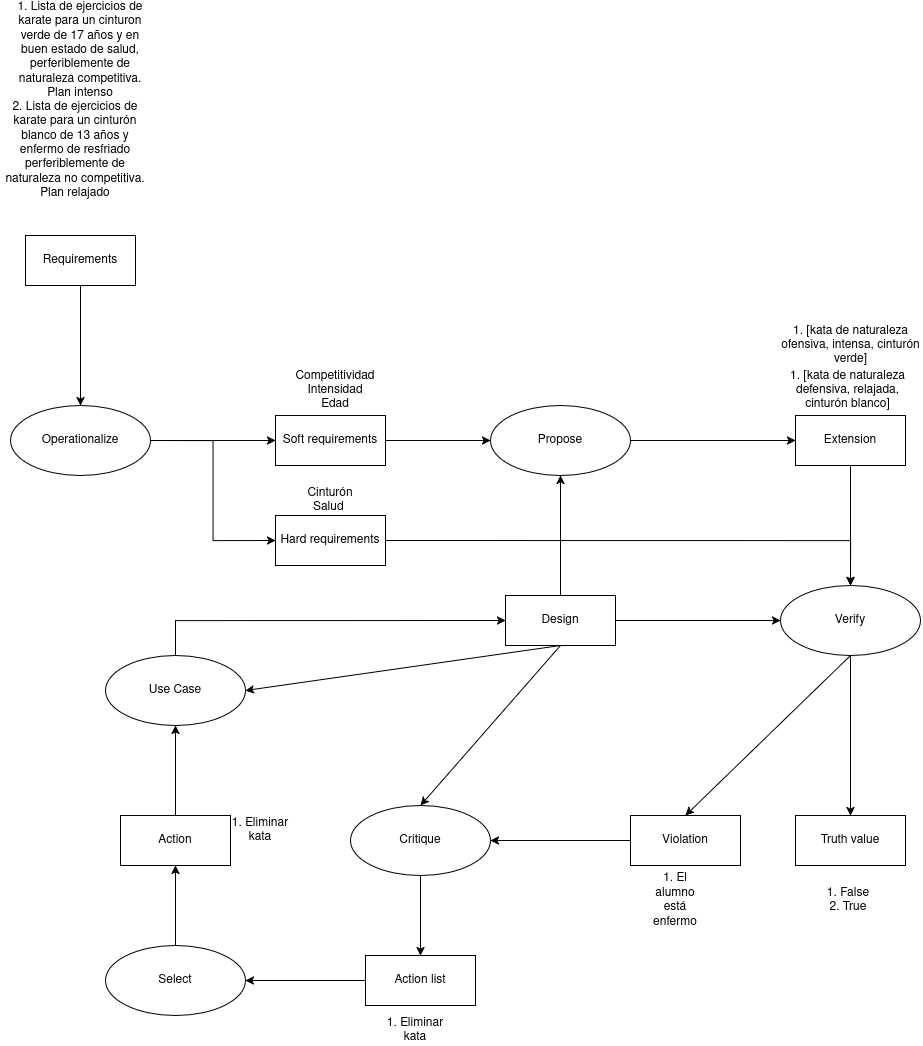
\includegraphics[width=\textwidth]{planotada}
\end{figure}

%%%%%%%%%%%%%%%%%%%%%%%%%%%%%%%%%%%%%%%%%%%%%%%%%%%%%%%%%%%%%%%%%%%%%%%%%%%%%%%
\subsubsection{Esquema inicial del dominio}
%%%%%%%%%%%%%%%%%%%%%%%%%%%%%%%%%%%%%%%%%%%%%%%%%%%%%%%%%%%%%%%%%%%%%%%%%%%%%%
\begin{figure}[H]
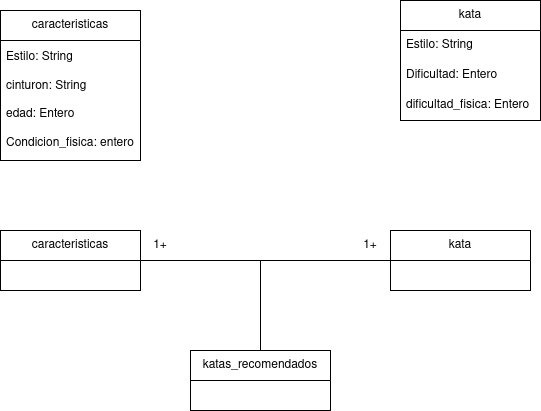
\includegraphics[width=\textwidth]{esqinicial}
\end{figure}
%%%%%%%%%%%%%%%%%%%%%%%%%%%%%%%%%%%%%%%%%%%%%%%%%%%%%%%%%%%%%%%%%%%%%%%%%%%%%%%
\subsubsection{Estructura inferencial y Mapeo}
%%%%%%%%%%%%%%%%%%%%%%%%%%%%%%%%%%%%%%%%%%%%%%%%%%%%%%%%%%%%%%%%%%%%%%%%%%%%%%
\begin{figure}[H]
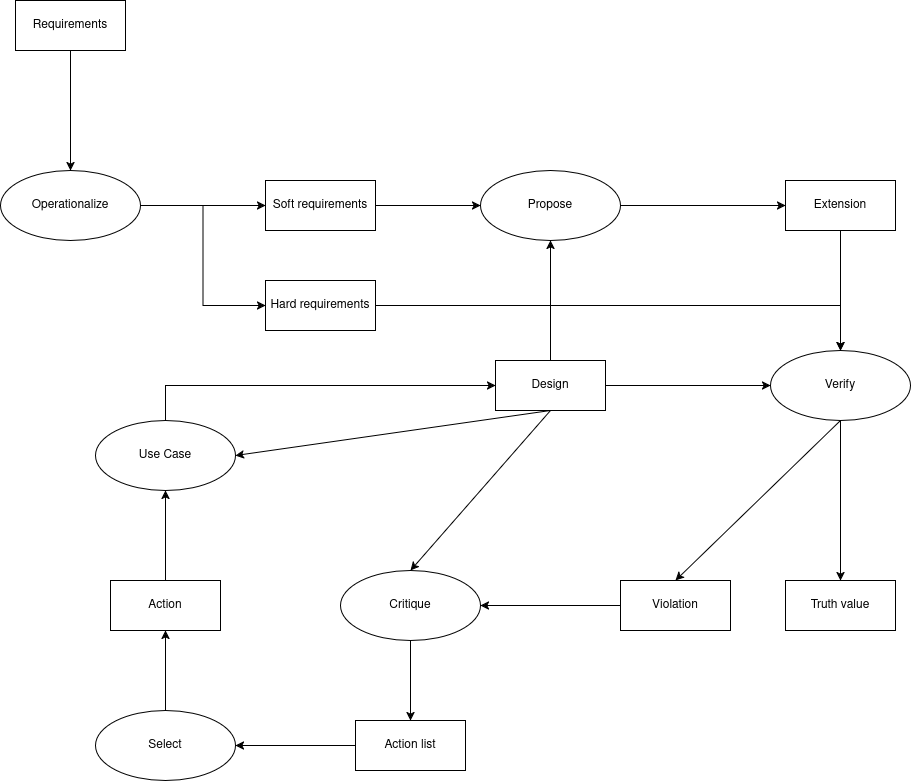
\includegraphics[width=\textwidth]{esinf}
\caption{Esquema inferencial modificado}
\end{figure}

\begin{figure}[H]
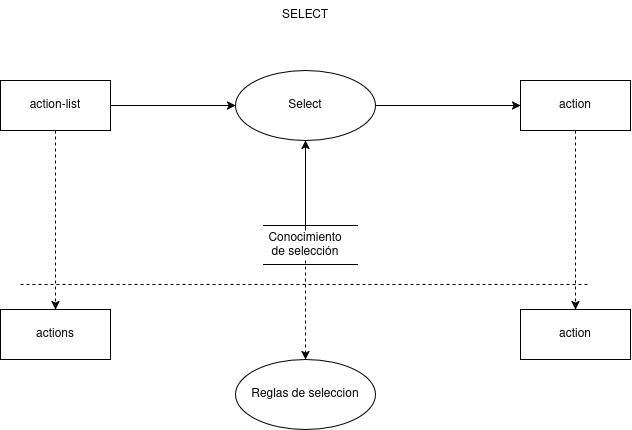
\includegraphics[width=\textwidth]{select}
\caption{Inferencia select}
\end{figure}

\begin{figure}[H]
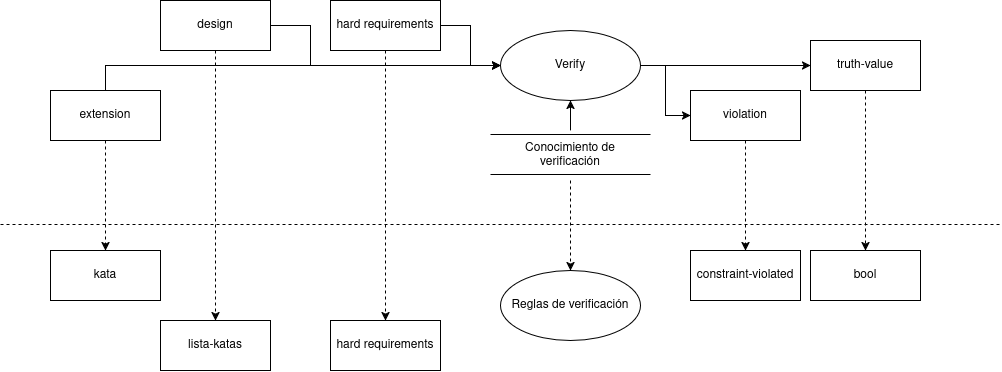
\includegraphics[width=\textwidth]{verify}
\caption{Inferencia verify}
\end{figure}

\begin{figure}[H]
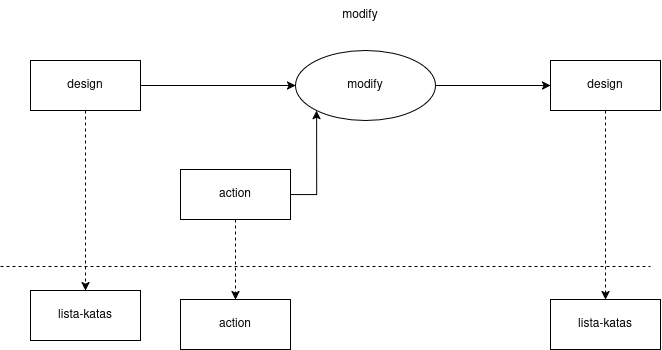
\includegraphics[width=\textwidth]{modify}
\caption{Inferencia modify}
\end{figure}

\begin{figure}[H]
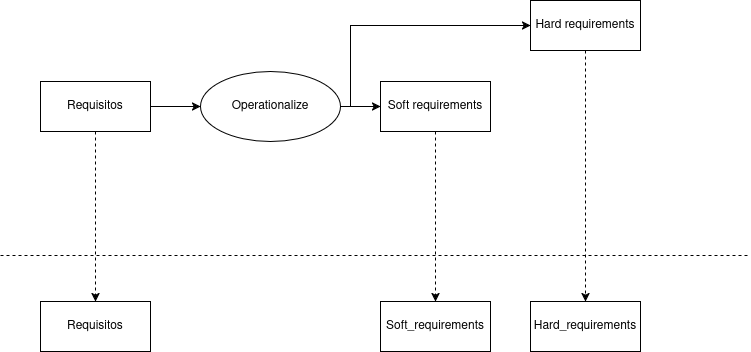
\includegraphics[width=\textwidth]{operacionalizar}
\caption{Inferencia operationalize}
\end{figure}

\begin{figure}[H]
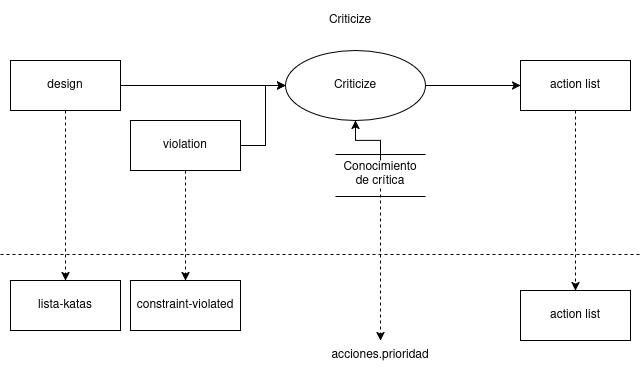
\includegraphics[width=\textwidth]{criticize}
\caption{Inferencia criticize}
\end{figure}

\begin{figure}[H]
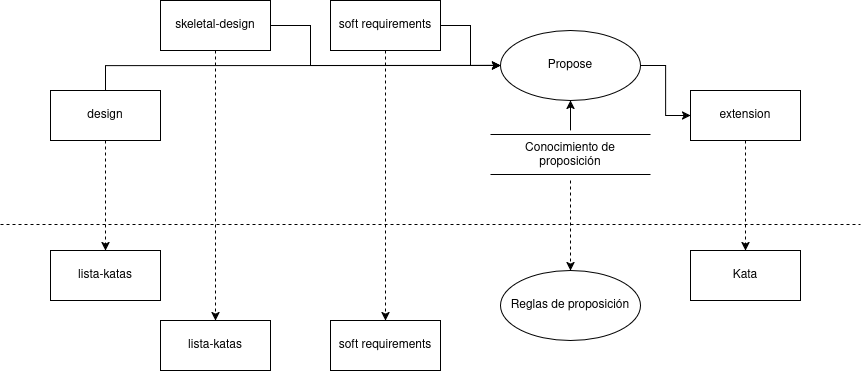
\includegraphics[width=\textwidth]{propose}
\caption{Inferencia propose}
\end{figure}

En la figura 5 podemos observar la inferencia operationalize, la cual, a partir de la entrada del usuario (en nuestro caso el Sensei)
convertirá los requisitos del usuario en restricciones (requisitos hard) y preferencias (requisitos soft).
En la figura 7 se presenta el rol estático propose, que, a través de reglas de proposición, las preferencias del sensei y el diseño ya presente,
propondrá un elemento a ser añadido a la lista de katas, la cual será verificada en la inferencia 3. La inferencia 3 emitirá 2 valores de salida dependiendo de la lista de katas actual: un valor bool dependiendo del cumplimiento de las restricciones, y emitirá una violación de no cumplir los requisitos.

Posterior a la verificación, la violación y la lista de katas extendida se introducirán en la inferencia criticize (Figura 6) y mediante conocimiento de crítica se dispondrá de una lista de acciones para devolver la lista de katas a un estado verificable. Utilizando el rol estático select (Figura 2) se seleccionará la acción mas apropiada, la cual se llevará a cabo en la inferencia modify (Figura 4). Una vez finalizado este proceso, se reintroducirá al proceso de verificación la lista de katas modificada.

%%%%%%%%%%%%%%%%%%%%%%%%%%%%%%%%%%%%%%%%%%%%%%%%%%%%%%%%%%%%%%%%%%%%%%%%%%%%%%% 
\subsubsection{Tarea}
%%%%%%%%%%%%%%%%%%%%%%%%%%%%%%%%%%%%%%%%%%%%%%%%%%%%%%%%%%%%%%%%%%%%%%%%%%%%%%
Especificación de la tarea (entradas y salidas) y Método de la tarea:
\begin{verbatim}
TASK configuration-design; 
    ROLES: 
        INPUT: requirements: "requisitos del diseño"; 
        OUTPUT: design: "diseño final resultante"; 
END TASK configuration-design; 

TASK-METHOD propose-and-revise; 
    REALIZES: configuration-design; 
    DECOMPOSITION: 
        INFERENCES: operationalize, propose, verify, criticize, select, modify; 
    ROLES: 
        INTERMEDIATE: 
            soft-requirements: "requisitos a ser usados como preferencia"; hard-requirements: "requisitos que son restricciones graves"; 
            extension: "una nueva instancia para el diseño"; 
            violation: "restricciones incumplidas por el diseño actual"; 
            truth-value: "booleano que indica el resultado de la verificación"; 
            action-list: "lista ordenada de posibles acciones solución"; 
            action: "una instancia de una acción de las posibles soluciones"; 
    CONTROL-STRUCTURE: 
        operationalize(requirements -> hard-requirements + soft-requirements); 
        WHILE NEW-SOLUTION propose(design + soft-requirements -> extension) 
        DO 
            design := extension ADD design; 
            verify(design + hard-requirements -> truth-value + violation); 
            IF truth-value == false 
            THEN criticize(violation + design -> action-list); 
                REPEAT 
                    select(action-list -> action); 
                    modify(design + action -> design); 
                    verify(design + hard-requirements -> truth-value + violation);
                UNTIL truth-value == true; 
                END REPEAT 
            END IF 
        END WHILE 
END TASK-METHOD propose-and-revise;
\end{verbatim}
%%%%%%%%%%%%%%%%%%%%%%%%%%%%%%%%%%%%%%%%%%%%%%%%%%%%%%%%%%%%%%%%%%%%%%%%%%%%%%%
\subsubsection{Esquema del dominio final}
%%%%%%%%%%%%%%%%%%%%%%%%%%%%%%%%%%%%%%%%%%%%%%%%%%%%%%%%%%%%%%%%%%%%%%%%%%%%%%
\begin{figure}[H]
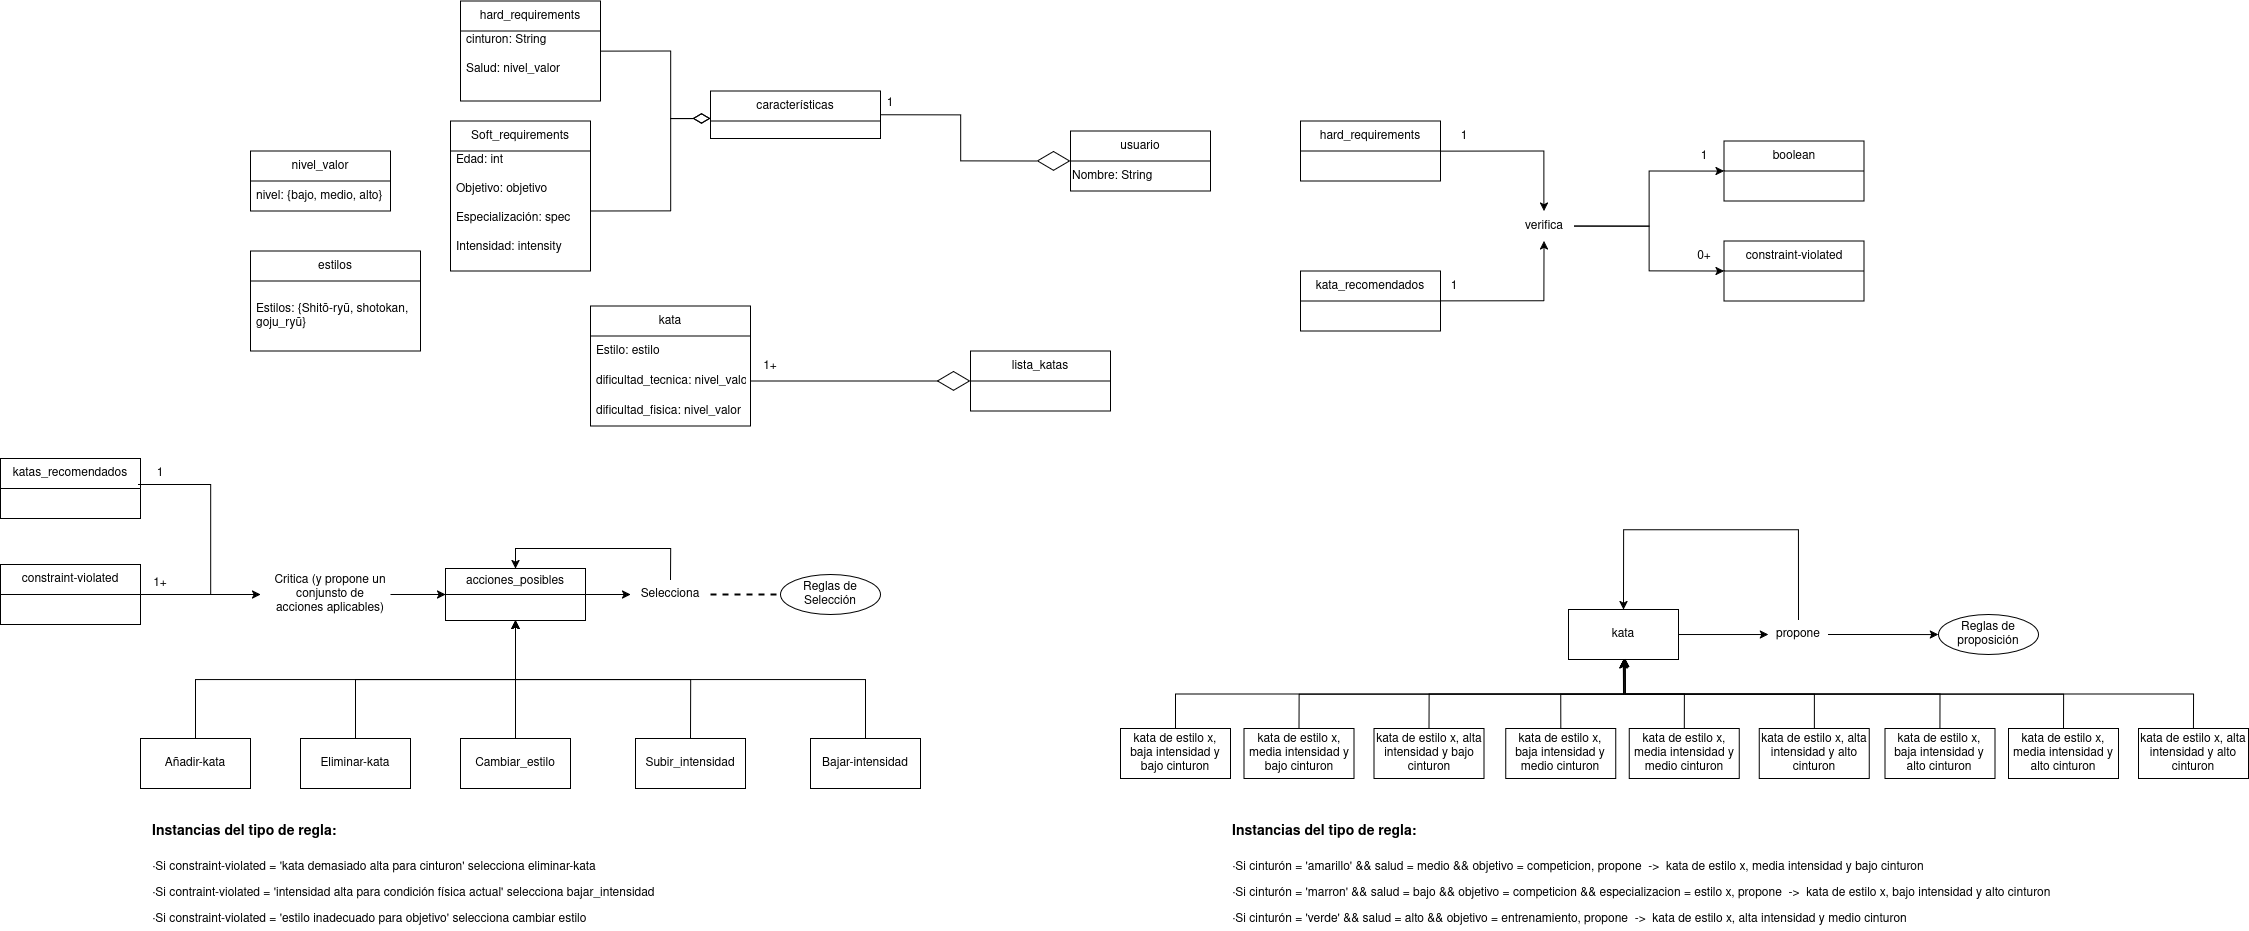
\includegraphics[width=\textwidth]{eidfinal}
\end{figure}
%%%%%%%%%%%%%%%%%%%%%%%%%%%%%%%%%%%%%%%%%%%%%%%%%%%%%%%%%%%%%%%%%%%%%%%%%%%%%%%
\subsection{Fase De Refinamiento}
%%%%%%%%%%%%%%%%%%%%%%%%%%%%%%%%%%%%%%%%%%%%%%%%%%%%%%%%%%%%%%%%%%%%%%%%%%%%%%%


%%%%%%%%%%%%%%%%%%%%%%%%%%%%%%%%%%%%%%%%%%%%%%%%%%%%%%%%%%%%%%%%%%%%%%%%%%%%%%%
\subsubsection{Validación}
%%%%%%%%%%%%%%%%%%%%%%%%%%%%%%%%%%%%%%%%%%%%%%%%%%%%%%%%%%%%%%%%%%%%%%%%%%%%%%

\textbf{Escenario 1.} El sensei le pide al sistema una "lista de ejercicios
para un cinturón verde de 17 años, sano, plan competitivo e intenso".

OPERATIONALIZE separa los requisitos: como hard quedan
\texttt{caracteristicas.cinturon = "verde"} y
\texttt{caracteristicas.salud = "buena"}, y como soft
\texttt{caracteristicas.edad = 17},
\texttt{caracteristicas.competitividad = "ofensiva"} e
\texttt{caracteristicas.intensidad = "alta"}. SPECIFY construye un
esqueleto del plan con los bloques habituales (calentamiento, kihon, kata,
kumite y vuelta a la calma) y PROPOSE lo rellena con ejercicios y una kata
de \texttt{kata.estilo = "shotokan"}, \texttt{kata.dificultad = "media"} y
\texttt{kata.dificultad\_fisica = "media"}, acordes al cinturón. VERIFY
revisa las restricciones del dominio (kata-cinturón y dificultad
física-salud) y no encuentra alarmas, así que CRITIQUE devuelve la lista
de acciones vacía y SELECT/MODIFY no llegan a ejecutarse. El plan sale
directamente al usuario.

\textbf{Escenario 2.} El sensei pide ahora una "lista de ejercicios para
un cinturón blanco de 13 años, con resfriado, plan no competitivo y
relajado".

OPERATIONALIZE deja como hard \texttt{caracteristicas.cinturon = "blanco"}
y \texttt{caracteristicas.salud = "enfermo:resfriado"}, y como soft la
edad, \texttt{caracteristicas.competitividad = "defensiva"} e
\texttt{caracteristicas.intensidad = "baja"}. SPECIFY ya quita el bloque
de kumite por la competitividad pedida. La primera pasada de PROPOSE, sin
embargo, no filtra del todo: mete una kata con \texttt{kata.estilo =
"shotokan"}, \texttt{kata.dificultad = "alta"} y
\texttt{kata.dificultad\_fisica = "alta"}, por encima del nivel del
alumno y con carga física incompatible con su salud.

VERIFY detecta entonces dos alarmas,
\texttt{alarma.mensaje = "La kata no corresponde a ese cinturón"} con
\texttt{alarma.dificultad = "alta"}, y \texttt{alarma.mensaje = "Carga
física no apta para el alumno"} con \texttt{alarma.dificultad\_fisica =
"alta"}. CRITIQUE las traduce en \{\texttt{sustituir-kata} (prioridad 1),
\texttt{reducir-dificultad-fisica} (prioridad 2)\}. SELECT coge la de
mayor prioridad y MODIFY cambia la kata por una de
\texttt{kata.dificultad = "baja"}. En la siguiente iteración VERIFY sigue
quejándose por la dificultad física, se aplica la segunda acción y en
una tercera pasada ya no hay alarmas, con lo que el plan se entrega.

Es este segundo caso el que justifica el bucle de refinamiento de la
plantilla: verify, critique, select y modify son los que dejan el plan
utilizable cuando la primera propuesta no lo está.




%Validación del modelo sobre los escenarios propuestos en la fase
%de identificación.

%%%%%%%%%%%%%%%%%%%%%%%%%%%%%%%%%%%%%%%%%%%%%%%%%%%%%%%%%%%%%%%%%%%%%%%%%%%%%%%
\subsubsection{Bases de conocimientos}
%%%%%%%%%%%%%%%%%%%%%%%%%%%%%%%%%%%%%%%%%%%%%%%%%%%%%%%%%%%%%%%%%%%%%%%%%%%%%%

Restricción kata-cinturón (la usa VERIFY):
\begin{verbatim}
RULE r-kata-cinturon-01;
  ANTECEDENT:
    kata.estilo = "shotokan" AND
    kata.dificultad = "alta" AND
    caracteristicas.cinturon = "blanco";
  CONSEQUENT:
    alarma.mensaje = "La kata no corresponde a ese cinturón" AND
    alarma.dificultad = "alta";
\end{verbatim}

Restricción dificultad física-salud (la usa VERIFY):
\begin{verbatim}
RULE r-kata-dificultad-fisica-01;
  ANTECEDENT:
    kata.dificultad_fisica = "alta" AND
    caracteristicas.salud = "enfermo:resfriado";
  CONSEQUENT:
    alarma.mensaje = "Carga fisica no apta para el alumno" AND
    alarma.dificultad_fisica = "alta";
\end{verbatim}
Reglas de PROPOSE
\begin{verbatim}
RULE r-propose-kata-competitivo;
  ANTECEDENT:
    caracteristicas.cinturon = "verde" AND
    caracteristicas.competitividad = "ofensiva";
  CONSEQUENT:
    kata.estilo = "shotokan" AND
    kata.dificultad = "media" AND
    kata.dificultad_fisica = "media";
\end{verbatim}

\begin{verbatim}
RULE r-propose-intensidad-alta;
  ANTECEDENT:
    caracteristicas.intensidad = "alta" AND
    caracteristicas.salud = "buena";
  CONSEQUENT:
    bloque.kihon = "tecnicas combinadas avanzadas" AND
    bloque.kumite = "combate libre (jiyu kumite)";
\end{verbatim}
Reglas de SELECT
\begin{verbatim}
RULE r-select-prioridad-tecnica;
  ANTECEDENT:
    acciones_disponibles = {sustituir-kata, reducir-dificultad-fisica} AND
    alarma.dificultad = "alta";
  CONSEQUENT:
    accion_elegida = sustituir-kata AND
    prioridad = 1;
\end{verbatim}

\begin{verbatim}
RULE r-select-prioridad-salud;
  ANTECEDENT:
    acciones_disponibles = {reducir-dificultad-fisica} AND
    caracteristicas.salud = "enfermo:resfriado";
  CONSEQUENT:
    accion_elegida = reducir-dificultad-fisica AND
    prioridad = 2;
\end{verbatim}
%Para estas prácticas, bastará con que las bases
%de conocimientos contengan TRES o CUATRO instancias de cada tipo de
%regla encontrado.

%%%%%%%%%%%%%%%%%%%%%%%%%%%%%%%%%%%%%%%%%%%%%%%%%%%%%%%%%%%%%%%%%%%%%%%%%%%%%%%
%%%%%%%%%%%%%%%%%%%%%%%%%%%%%%%%%%%%%%%%%%%%%%%%%%%%%%%%%%%%%%%%%%%%%%%%%%%%%%%
\section{Modelo de Comunicación}
%%%%%%%%%%%%%%%%%%%%%%%%%%%%%%%%%%%%%%%%%%%%%%%%%%%%%%%%%%%%%%%%%%%%%%%%%%%%%%%
%%%%%%%%%%%%%%%%%%%%%%%%%%%%%%%%%%%%%%%%%%%%%%%%%%%%%%%%%%%%%%%%%%%%%%%%%%%%%%%

%El modelado conceptual no está completo sin el modelo de
%comunicación, que es necesario realizar antes de la implementación. El
%modelo se realizará siguiendo las pautas de la metodología CommonKADS
%resumidas en la tabla 9.8 y se comprobará su corrección con respecto a los
%otros modelos ya construidos siguiendo las guías que se proporcionan en el
%apartado 9.7.4 del libro. En el documento a entregar se incluirán
%comentarios BREVES que demuestren que se han tenido en cuenta estos
%aspectos.

%%%%%%%%%%%%%%%%%%%%%%%%%%%%%%%%%%%%%%%%%%%%%%%%%%%%%%%%%%%%%%%%%%%%%%%%%%%%%%%
\subsection{Plan de comunicación general}
%%%%%%%%%%%%%%%%%%%%%%%%%%%%%%%%%%%%%%%%%%%%%%%%%%%%%%%%%%%%%%%%%%%%%%%%%%%%%%

%Brevemente COMENTADO y que incluya:
%\begin{itemize}
% \item Diagrama de diálogo
% \item Información de control de las transacciones en forma de
%seudocódigo o de diagrama de transición
%\end{itemize}
Para la tarea que hemos desarrollado las comunicaciones se producen entre el diseñador y el SBC y el SBC y la base de datos.
El diseñador especificará los requisitos al sistema y seleccionará acciones en el caso de que la solución parcial no cumpla los
requisitos. Por otro lado, al final del procesamiento el SBC se comunicará con la base de datos para guardar la solución.

\begin{figure}[H]
  \includegraphics[width=\textwidth]{diagramadial}
  \caption{Diagrama de diálogo}
\end{figure}

\begin{figure}[H]
  \includegraphics[width=\textwidth]{diagramatrans}
  \caption{Diagrama de transición}
\end{figure}
%%%%%%%%%%%%%%%%%%%%%%%%%%%%%%%%%%%%%%%%%%%%%%%%%%%%%%%%%%%%%%%%%%%%%%%%%%%%%%%
\subsection{Descripción de las Transacciones}
%%%%%%%%%%%%%%%%%%%%%%%%%%%%%%%%%%%%%%%%%%%%%%%%%%%%%%%%%%%%%%%%%%%%%%%%%%%%%%

\begin{table}[H]
\centering
\label{tab:cm1}
 
\begin{tabularx}{\textwidth}{|X|X|}
\hline
\textbf{Modelo de Comunicación} & \textbf{Hoja de Trabajo de Descripción de Transacción CM-1} \\
\hline
 
IDENTIFICADOR/NOMBRE DE TRANSACCIÓN & TR1: Introducir requisitos \\
\hline
 
OBJETO DE INFORMACIÓN & Lista de restricciones y preferencias (Especialización, competitividad, nivel...) deseados para el plan por el sensei.
\\
\hline
 
  AGENTES INVOLUCRADOS & Agente emisor: Sensei \newline Agente receptor: SBC
  \\ 
\hline
 
PLAN DE COMUNICACIÓN & 
\\
\hline
 
RESTRICCIONES & Debe existir una lista de katas vacía.
\\
\hline
 
ESPECIFICACIÓN DE INTERCAMBIO DE INFORMACIÓN & Tipo ORDER (Predefinido en el libro Schreiber)
\\
\hline
 
\end{tabularx}
 
\end{table}

\begin{table}[H]
\centering
\label{tab:cm1}
 
\begin{tabularx}{\textwidth}{|X|X|}
\hline
\textbf{Modelo de Comunicación} & \textbf{Hoja de Trabajo de Descripción de Transacción CM-1} \\
\hline
 
IDENTIFICADOR/NOMBRE DE TRANSACCIÓN & TR2: Seleccionar acción \\
\hline
 
OBJETO DE INFORMACIÓN & Lista de acciones aplicables a una lista de katas con katas mal introducidas (que incumplan preferencias o requisitos)
\\
\hline
 
AGENTES INVOLUCRADOS & Agente emisor: SBC (Digo yo que si pero no estoy seguro -dza) \newline Agente Receptor: Diseñador
  \\ 
\hline
 
PLAN DE COMUNICACIÓN & 
\\
\hline
 
RESTRICCIONES & Se da cuando el SBC detecta elementos mal introducidos en la lista de katas
\\
\hline
 
ESPECIFICACIÓN DE INTERCAMBIO DE INFORMACIÓN & Tipo ASK/REPLY (Predefinido en el libro Schreiber)
\\
\hline
 
\end{tabularx}
 
\end{table}

\begin{table}[H]
\centering
\caption{Hoja de Trabajo CM-1: Descripción de Transacción}
\label{tab:cm1}
 
\begin{tabularx}{\textwidth}{|X|>{\raggedright\arraybackslash}X|}
\hline
\textbf{Modelo de Comunicación} & \textbf{Hoja de Trabajo de Descripción de Transacción CM-1} \\
\hline
 
IDENTIFICADOR/NOMBRE DE TRANSACCIÓN & TR3.1: Mostrar solución \\
\hline
 
OBJETO DE INFORMACIÓN & Lista de katas con todos los elementos ya insertados correctamente
\\
\hline
 
AGENTES INVOLUCRADOS & Agente emisor: SBC \newline Agente Receptor: Sensei
  \\ 
\hline
 
PLAN DE COMUNICACIÓN & 
\\
\hline
 
RESTRICCIONES & El SBC ha de disponer de una solución que cumpla con los requisitos. 
\\
\hline
 
ESPECIFICACIÓN DE INTERCAMBIO DE INFORMACIÓN & Tipo REPORT (Predefinido en el libro Schreiber)
\\
\hline
 
\end{tabularx}
 
\end{table}


\begin{table}[H]
\centering
\label{tab:cm1}
 
\begin{tabularx}{\textwidth}{|X|X|}
\hline
\textbf{Modelo de Comunicación} & \textbf{Hoja de Trabajo de Descripción de Transacción CM-1} \\
\hline
 
IDENTIFICADOR/NOMBRE DE TRANSACCIÓN & TR3.2: Guardar solución \\
\hline
 
OBJETO DE INFORMACIÓN & Lista de katas con todos los elementos ya insertados correctamente
\\
\hline
 
  AGENTES INVOLUCRADOS & Agente emisor: SBC \newline Agente Receptor: Base de datos
  \\ 
\hline
 
PLAN DE COMUNICACIÓN & 
\\
\hline
 
RESTRICCIONES & El SBC ha de disponer de una solución que cumpla con los requisitos. 
\\
\hline
 
ESPECIFICACIÓN DE INTERCAMBIO DE INFORMACIÓN & Tipo REPORT (Predefinido en el libro Schreiber)
\\
\hline
 
\end{tabularx}
 
\end{table}
%%%%%%%%%%%%%%%%%%%%%%%%%%%%%%%%%%%%%%%%%%%%%%%%%%%%%%%%%%%%%%%%%%%%%%%%%%%%%%%
\subsection{Especificación de las transacciones}
%%%%%%%%%%%%%%%%%%%%%%%%%%%%%%%%%%%%%%%%%%%%%%%%%%%%%%%%%%%%%%%%%%%%%%%%%%%%%%
Ya que hemos empleado los tipos de transacciones ya predefinidos en el libro de Schreiber no hemos definido ninguna nueva transacción.
%%Modelo CM-2 para las transacciones identificadas. 
%%
%%\textbf{NOTA IMPORTANTE:} Normalmente los modelos de comunicación de las prácticas son sencillos, por lo que este formulario puede no ser necesario. Se realizará sólo
%%para las transacciones complejas que no queden completamente
%%especificadas con el modelo CM-1.
%%%%%%%%%%%%%%%%%%%%%%%%%%%%%%%%%%%%%%%%%%%%%%%%%%%%%%%%%%%%%%%
%FINAL DEL LIBRO
%%%%%%%%%%%%%%%%%%%%%%%%%%%%%%%%%%%%%%%%%%%%%%%%%%%%%%%%%%%%%%%
\end{document}
